
Multiparameter Persistence (often referred to as Multipersistence) introduces a novel concept with the potential to significantly enhance the performance of single-parameter persistence. The concept, introduced in the late 2000s by Carlsson, Zomorodian, and Singh~\cite{carlsson2007theory,carlsson2009computing}, has since been actively investigated for real-world applications~\cite{botnan2022introduction}.



\begin{wraptable}{r}{6cm}
\vspace{-.1in}
\caption{Generic Bifiltration \label{tab:bifiltration}}
\resizebox{1.\linewidth}{!}{
\begin{tabular}{ccccccc}
$\K_{m1}$ & $\subset$ & $\K_{m2}$ & $\subset$ & $\dots$ & $\subset$ & $\K_{mn}$ \\
$\cup$ &  & $\cup$ &  & $\cup$ &  & $\cup$\\
$\dots$ & $\subset$ & $\dots$ & $\subset$ & $\dots$ & $\subset$ & $\dots$\\
$\cup$ &  & $\cup$ &  & $\cup$ &  & $\cup$\\
$\K_{21}$ & $\subset$ & $\K_{22}$ & $\subset$ & $\dots$ & $\subset$ & $\K_{2n}$ \\
$\cup$ &  & $\cup$ &  & $\cup$ &  & $\cup$\\
$\K_{11}$ & $\subset$ & $\K_{12}$ & $\subset$ & $\dots$ & $\subset$ & $\K_{1n}$ \\
\end{tabular}}
\vspace{-.1in}
\end{wraptable}

 
For original PH, the term \textit{single persistence} is applied because we filter the data in just one direction, $\K_1\subset \K_2\subset\dots\subset\K_n$. The filtration's construction is pivotal in achieving a detailed analysis of the data to uncover hidden shape patterns. For example, for graph setting, when utilizing a single function $f:\V\to\R$ containing crucial domain information (e.g., value for blockchain networks, atomic number for protein networks), it induces a single-parameter filtration as described earlier. However, numerous datasets offer multiple highly relevant domain functions for data analysis. Similarly, in other data types, there are several ways to expand the single filtration into multifiltration to get finer information on the topological patterns hidden in the data. The idea of using multiple filtration functions simultaneously to obtain a finer decomposition of the dataset led to the suggestion of the MP theory as a natural extension of single persistence (SP).

 
 
\subsection{Multifiltrations} 

Multifiltration refers to filtrations constructed using multiple scale parameters. A typical example of a bifiltration, denoted as $\{\K_{ij}\}$, is illustrated in Table~\ref{tab:bifiltration}, where each row and column corresponds to a distinct filtration. This bifiltration is generated by simultaneously varying one scale parameter along the horizontal axis and another along the vertical axis. The specific construction of these filtrations depends on the data type, with additional parameters introduced based on the nature of the data. Below, we summarize common methods for different data types. While the explanation focuses on two parameters for simplicity, this approach generalizes to any number of parameters.

\begin{figure}[b]
    \centering
    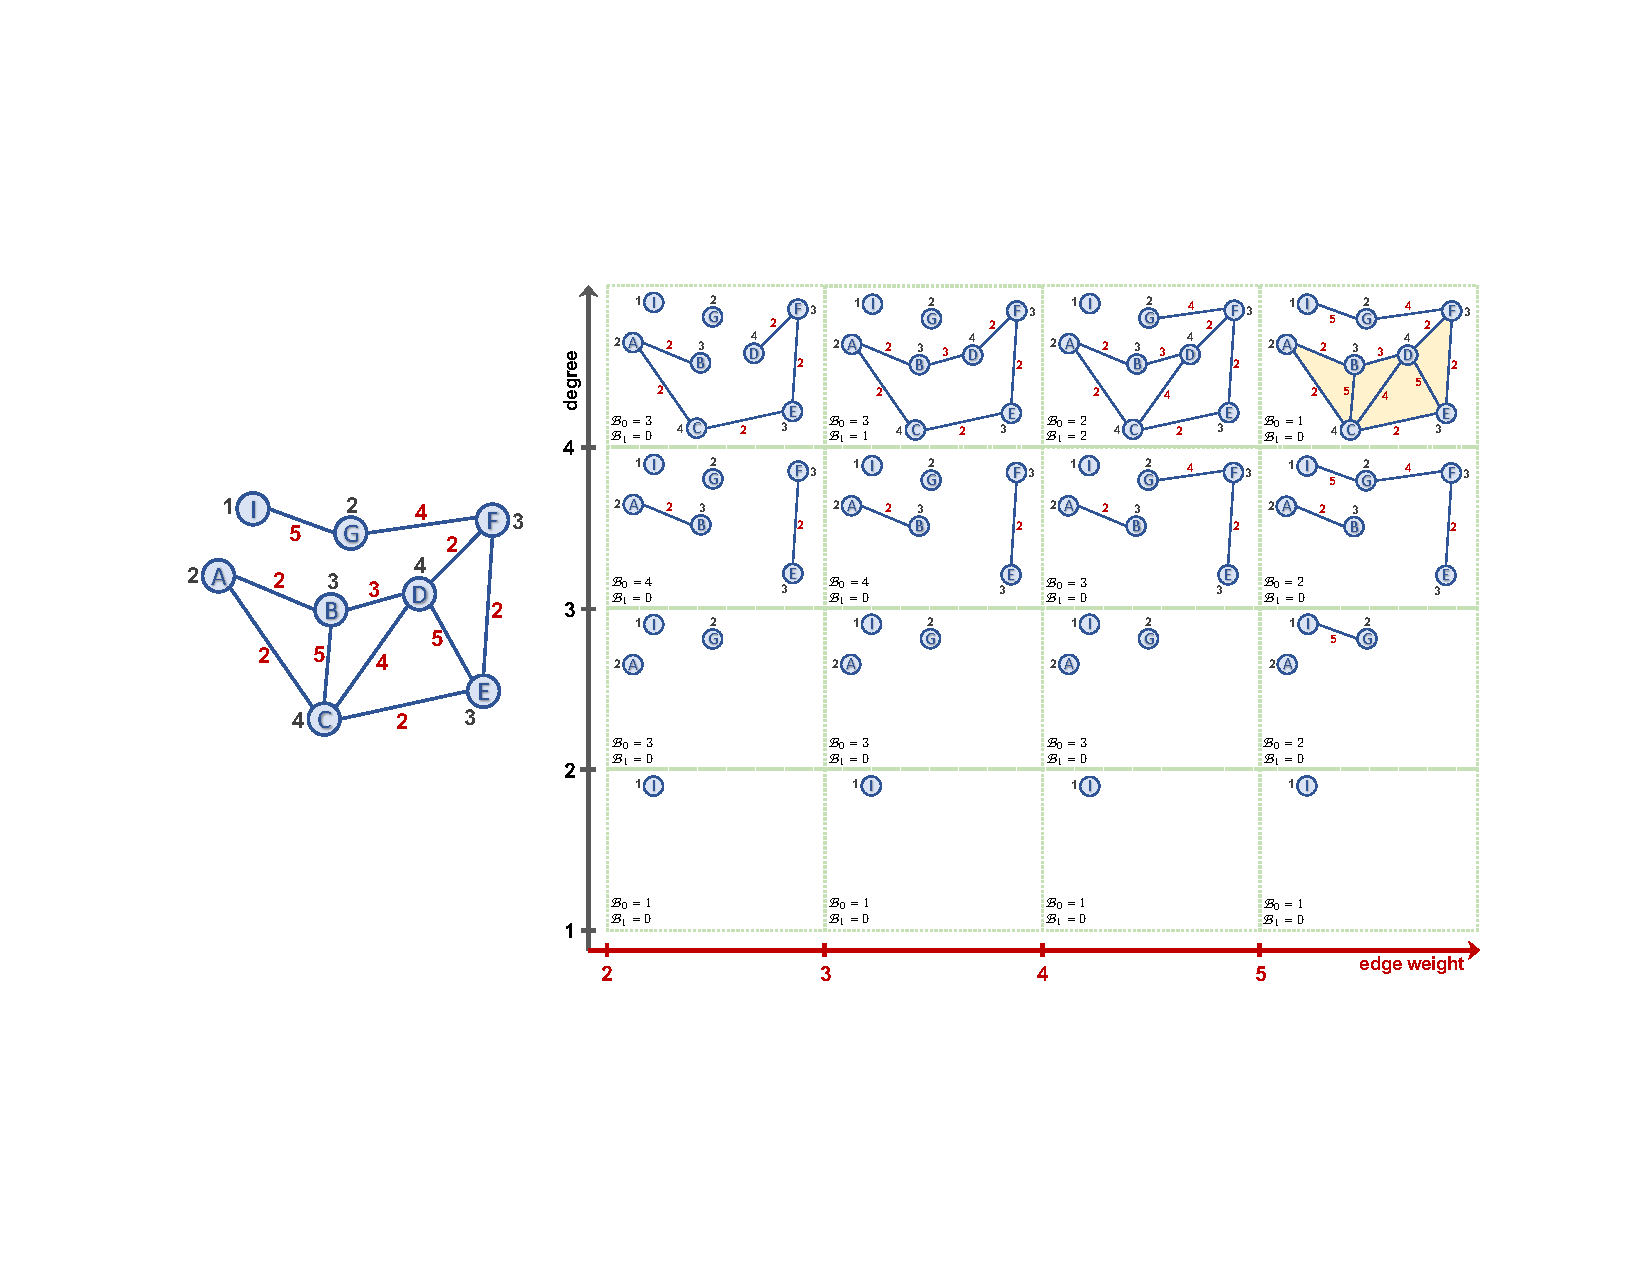
\includegraphics[width=.9\textwidth]{figures/MP_Example.pdf}
    \caption{\footnotesize Multidimensional persistence on a graph network (original graph: left). Black numbers denote the degree values of each node whilst red numbers show the edge weights of the network. Hence, shape properties are computed on two filtration functions (i.e., degree and edge weight). While each row filters by degree, each column filters the corresponding subgraph using its edge weights. For each cell, the lower left corners represent the corresponding threshold values. For each cell, $\mathcal{B}_{0}$ and $\mathcal{B}_{1}$ represent the corresponding Betti numbers. The figure is adapted from~\cite{chen2024emp}. \label{Fig:ToyMP}}
\end{figure}
 
\subsubsection{Multifiltrations for Graphs.} \label{sec:MP-graph}

In graph settings, a single filtration function results in a single-parameter filtration $\wh{\G}_1 \subset \dots \subset \wh{\G}_N = \wh{\G}$. However, employing multiple filtration functions enables a more detailed analysis of the data. For instance, two node functions $f: \V \to \R$ and $g: \V \to \R$, which provide complementary information about the network, can be combined using Multiparameter Persistence to generate a unique topological fingerprint. These functions induce a multivariate filtration function $F: \V \to \R^2$ defined by $F(v) = (f(v), g(v))$.

Next, we define sets of increasing thresholds $\{\alpha_i\}_{i=1}^m$ for $f$ and $\{\beta_j\}_{j=1}^n$ for $g$. Then, we have $\V_{ij} = \{v_r \in \V \mid f(v_r) \leq \alpha_i, g(v_r) \leq \beta_j\}$, which can be written as $\V_{ij} = F^{-1}((-\infty, \alpha_i] \times (-\infty, \beta_j])$. Let $\G_{ij}$ be the subgraph of $\G$ induced by $\V_{ij}$, meaning the smallest subgraph of $\G$ generated by $\V_{ij}$. This setup induces a bifiltration of complexes $\{\wh{\G}_{ij} \mid 1 \leq i \leq m, 1 \leq j \leq n\}$, which can be visualized as a rectangular grid of size $m \times n$ (see \cref{Fig:ToyMP}). For more details on applying multipersistence in graph settings, refer to \cite{chen2024emp, loiseaux2024stable}. Additionally, one can combine power filtration with filtration by functions by applying power filtration to each subgraph in the sequence induced by sublevel filtration via functions~\cite{demir2022todd}. In \Cref{sec:drug}, we give details of the utilization of MP method on graph setting for computer-aided drug discovery.



\subsubsection{Multifiltrations for Point Clouds.} \label{sec:MP-point_cloud}

In the context of point clouds, a natural parameter to consider is the radius $r$, as discussed in~\Cref{sec:point_cloud}. However, a point cloud $\p$ often has regions of varying density, with some areas being very dense and others quite sparse. Additionally, a few outliers can significantly distort the topological signature due to the way it is constructed. To address this issue, it is common to use a density parameter in conjunction with the radius parameter when constructing the filtration. This parameter reflects the local density of points in the point cloud and helps identify regions of different densities, distinguishing features significant in dense regions from those in sparse ones.
To achieve this, we first need to compute local densities. For each point $p \in \p$, we compute a density measure $\delta(p)$, which could be based on the number of points within a fixed radius $r_d$ or kernel density estimation~\cite{vipond2020multiparameter,botnan2022introduction}.
 

Next, we define our threshold set $\{(d_i, r_j)\}$, where $d_1 > d_2 > \dots > d_m$ corresponds to thresholds for density, and $0 = r_1 < r_2 < \dots < r_n = \text{diam}(\p)$ are radius thresholds. We then define the multifiltration as follows. Using $\delta(p)$, we define a nested sequence of subsets $\p_1 \subset \p_2 \subset \dots \subset \p_m = \p$, where $\p_i = \{p \in \p \mid \delta(p) \geq d_i\}$. For each $i_0$, we treat $\p_{i_0}$ as a separate point cloud and apply the Rips filtration process to it. Specifically, for each $i_0$, we construct the Rips filtration $\VR_{i_01} \subset \VR_{i_02} \subset \dots \subset \VR_{i_0n}$. This gives a bifiltration $\{\K_{ij}\}$ as in \Cref{tab:bifiltration}, with $\K_{ij} = \VR_{ij}$ representing the Rips filtration for point cloud $\p_i$ with radius parameter $r_j$. e.g., the first column $\K_{i1} = \p_i$ corresponds to radius $r_1 = 0$.

This multifiltration approach provides more detailed information by capturing topological patterns in both dense and sparse regions, offering a richer understanding of the data's underlying shape, especially when varying densities and scales are crucial for the analysis. For further details, see~\cite{loiseaux2024framework,vipond2020multiparameter}.

\subsubsection{Multifiltrations for Images.} \label{sec:MP-image}

Similarly, in the image setting, if the image is a color image, one can easily employ all color channels at the same time, similar to the graph setting. In particular, a color image has three color functions, denoted as $R$ (red), $G$ (green), and $B$ (blue). Thus, for every pixel $\Delta_{ij}$, there exist corresponding color values: $R_{ij},G_{ij},B_{ij}\in [0,255]$. To proceed, we establish a three-parameter multifiltration with parameters $\{\alpha_m\}_1^{N_R}$, $\{\beta_n\}_1^{N_G}$, $\{\gamma_r\}_1^{N_B}$, where $\alpha_m,\beta_n,\gamma_r\in [0,255]$ are threshold values for color channels $R,G$, and $B$ respectively. By simply defining binary images $\X_{m,n,r}=\{\Delta_{ij}\subset \X \mid  R_{ij}\leq \alpha_m, G_{ij}\leq \beta_n, B_{ij}\leq \gamma_r\}$, we obtain a three parameter multifiltration of size $N_R \times N_G \times N_B$.
Similarly, for grayscale images, one can utilize height, radial, erosion, signed distance, or similar filtration methods~\cite{garin2019topological} along with the color filtration to obtain a multifiltration for color images.



\subsection{MP Vectorization Methods} \label{sec:MP-vec}

By computing the homology groups of the complexes in these multifiltrations, $\{\h_k(\K_{ij})\}$, along with the induced inclusion maps, we obtain the corresponding \textit{multipersistence module}, which can be visualized as a rectangular grid of size $m\times n$. The goal here is to track $k$-dimensional topological features through the homology groups $\{\h_k(\K_{ij})\}$ within this grid. However, as explained in~\cite{botnan2022introduction}, technical challenges rooted in commutative algebra prevent us from transforming the multipersistence module into a mathematical structure like a "Multipersistence Diagram." The key issue is that for any $k$-dimensional hole in the multifiltration, we cannot directly assign a birth and death time due to the partial ordering within the module. For example, if the same $k$-hole $\sigma$ appears at $\K_{1,4}$ and $\K_{2,3}$, neither $(1,4) \nprec (2,3)$ nor $(2,3) \nprec (1,4)$, making it difficult to define a birth or death time for $\sigma$ unless it exists in a perfectly rectangular region. This issue does not arise in single persistence, where any two indices are always comparable, i.e., $i<j$ or $j<i$.

As a result, we do not have an effective representation of the MP module~\cite{botnan2022introduction}. While these technical obstacles prevent this promising approach from reaching its full potential in real-life applications, in the past years, several approaches have been proposed to extract key insights from MP modules by skipping MP representations and directly going to the vectorization from multifiltrations, which we detail below. 



The simplest method to derive a vector (or tensor) from a multifiltration involves using the \textit{Hilbert function} of the MP module, which is a generalization of Betti functions. Let $\{\K_{ij}\}$ denote an $m \times n$ multifiltration associated with a given dataset $\X$. First, we construct the multipersistence module ${\h_k(\K_{ij})}$. Next, by computing the Betti numbers of each simplicial complex in the multifiltration, we obtain an $m \times n$ matrix (or tensor) $\wh{\beta}_k(\X) = [\beta_k(\K{ij})]$, i.e., $\beta_k(\K_{ij}) = \text{rank}(\h_k(\K_{ij}))$. These are also called \textit{multipersistence (or bigraded) Betti numbers}. In graph representation learning, this simple vectorization of the MP module has demonstrated remarkable performance~\cite{loiseaux2024stable,chen2024emp,xin2023gril}.



While bigraded Betti numbers offer a straightforward vectorization method for multiparameter (MP) modules, they fail to capture crucial topological information, especially regarding the significance of dominant features or the presence of a few important topological features. More sophisticated techniques are necessary for effective MP vectorization. One widely used strategy involves the "slicing technique," which focuses on studying one-dimensional fibers within the multiparameter domain. A clearer understanding can be obtained by restricting the multidimensional persistence module to these single directions (slices) and applying single persistence analysis. 

In their work \cite{carriere2020multiparameter}, Carriere et al. explored this approach by considering multiple such slices, often referred to as {\em vineyards}, and summarizing the resulting persistence diagrams. Another significant advancement is found in {\em multipersistence landscapes} \cite{vipond2020multiparameter} by Vipond, which extends the concept of persistence landscapes \cite{bubenik2015statistical} from single to multiparameter persistence. 

The vectorization of MP modules is a rapidly evolving area of research. Various techniques have recently been proposed in practical applications, e.g.,  Hilbert decomposition signed measure (MP-HSM-C)~\cite{loiseaux2024stable}, Effective MultiPersistence (EMP)~\cite{chen2024emp}, Generalized Rank Invariant Landscape (GRIL)~\cite{xin2023gril}, and Stable Candidate Decomposition Representations (S-CDR)~\cite{loiseaux2024framework}. Although many recent methods are burdened by high computational costs, the MP-HSM-C method introduced by Loiseaux et al.~\cite{loiseaux2024stable} stands out as the most efficient in terms of speed and performance among current MP vectorization techniques.
 



